\documentclass[12pt]{article}
\usepackage{amsthm}
\usepackage{amsmath}
\usepackage{array}
\usepackage{cancel}
\usepackage[thinc]{esdiff}
% \usepackage{gensymb}
\usepackage{geometry}
\usepackage{graphicx}
\usepackage{pgfplots}
\usepackage{siunitx}
\usepackage{wrapfig}
\usepackage{xcolor}

\title{Chapter 1 Problems, MIT 8.03}
\author{Donald Aingworth IV}
\date{Feast of Peter and Paul 2025}

\pgfplotsset{width=8cm,compat=1.9}
\usepgfplotslibrary{external}
% \tikzexternalize

\renewcommand\thesubsection{\alph{subsection}}
\newcommand{\proj}{\text{proj}}
\newtheorem{theorem}{Theorem}

\begin{document}

\DeclareSIUnit{\mile}{mi}
\DeclareSIUnit{\gal}{gal}
\DeclareSIUnit{\foot}{ft}
\DeclareSIUnit{\hour}{h}
\DeclareSIUnit{\rad}{rad}
\DeclareSIUnit{\unit}{u}
\DeclareSIUnit{\dyne}{dyn}

\maketitle

\pagebreak
\section{Problem 1}
For the mass and spring discussed (1.1)-(1.8), suppose that the system is hung vertically in the earth’s gravitational field, with the top of the spring held fixed. Show that the frequency for vertical oscillations is given by (1.5). Explain why gravity has no effect on the angular frequency.
% \begin{wrapfigure}{r}{0.25\textwidth}
%     \vspace{-30pt}
%     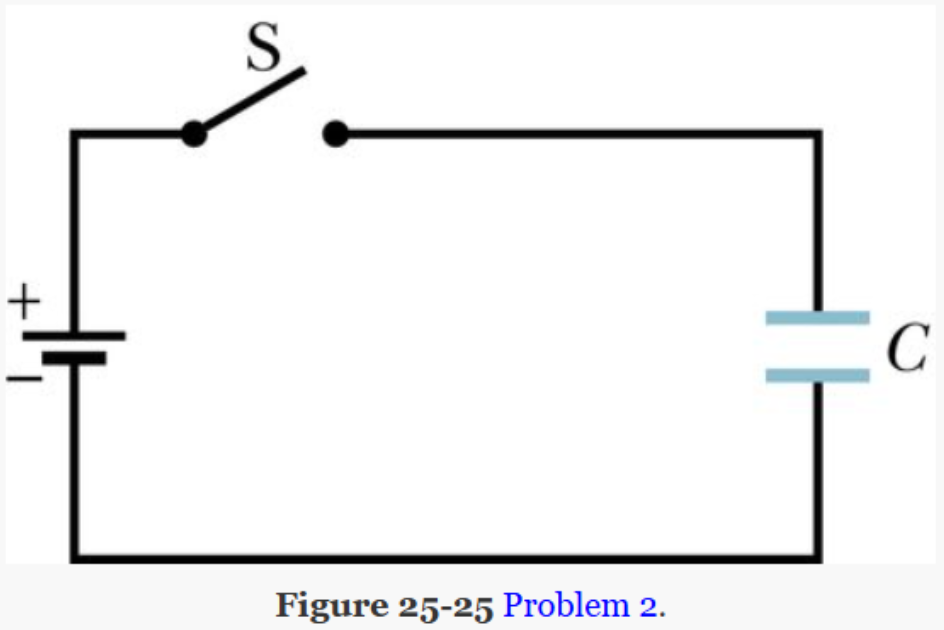
\includegraphics[width=0.25\textwidth]{picture_1.png} 
%     % \label{fig:wrapfig}
% \end{wrapfigure}


\subsection*{Solution}
Besides unconsidered statics, the only forces on the object are in the vertical ($\hat{y}$) directon. 
\begin{gather}
    \vec{F}_{net} = \vec{F}_s - \vec{F}_g = -kx(t) \hat{y} - mg\hat{y} = m\vec{a}\\
    mx''(t) + kx(t) = -mg
\end{gather}

This gives us a differential equation.
Since \(-mg\) contains no reference to $x(t)$ and is made up of only constants, we can ignore it for the moment.
This is a common practice when solving ordinary differential equations.
\begin{gather}
    mx''(t) + kx(t) = 0\\
    x''(t) + \frac{k}{m}x(t) = 0\\
    x''(t) = -\frac{k}{m}x(t)
\end{gather}

This is a simple second order differential equation to solve, so we can skip over it.
\begin{equation}
    x(t) = x_0 \cos\left(\sqrt{\frac{k}{m}}t + \phi\right)
\end{equation}

This derives why it is that \(\omega = \sqrt{\frac{k}{m}}\).
In this case, gravity is applied constantly and consistently, so why it may affect the initial problem with reference to the ground, it wll not change the oscillation over time or the position with reference to the center of the oscillation.

\pagebreak
\section{Problem 2}
a. Find an expression for $\cos(7\theta)$ in terms of $\cos(\theta)$ and $\sin(\theta)$ by using complex exponentials and the binomial expansion.\\
b. Do the same for $\sin(5\theta)$.\\
c. Use complex exponentials to find an expression for $\sin(\theta_1 + \theta_2 + \theta_3)$ in terms of the sines and cosines of the individual angles.\\
d. Do you remember the “half angle formula,”
\[ \cos^2\frac{\theta}{2} = \frac{1}{2}(1 + \cos(\theta)) ?\]
Use complex exponentials to prove the “fifth angle formula,”
\[ \cos^5 \frac{\theta}{5} = \frac{10}{16}\cos\frac{\theta}{5} + \frac{5}{16}\cos\frac{3\theta}{5} + \frac{1}{16}\cos\theta \]
e. Use complex exponentials to prove the identity
\[ \sin 6x = \sin x \left( 32\cos^5 x - 32\cos^3 x + 6\cos x \right) \]

% \begin{wrapfigure}{r}{0.25\textwidth}
%     \vspace{-30pt}
%     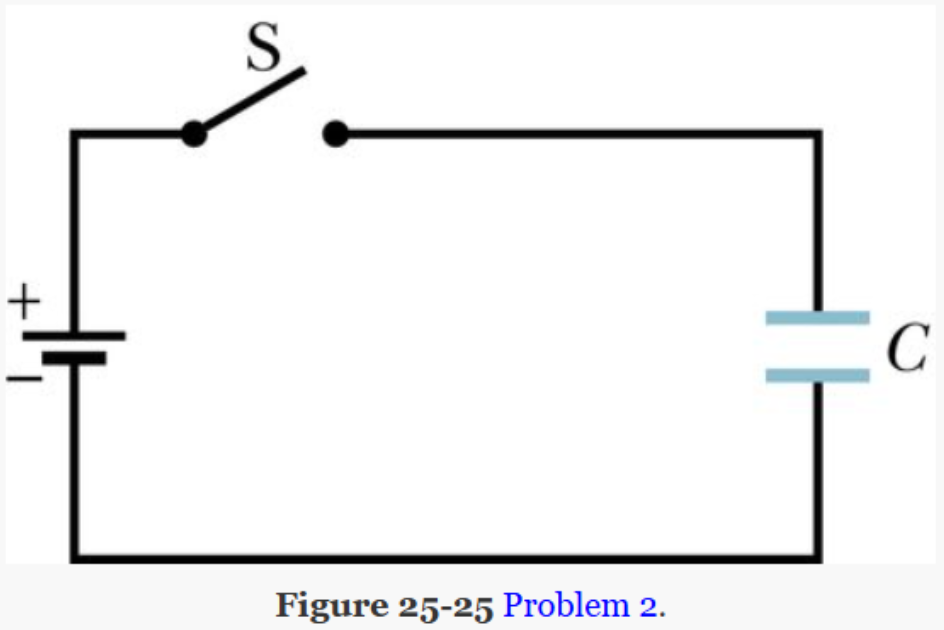
\includegraphics[width=0.25\textwidth]{picture_1.png} 
%     % \label{fig:wrapfig}
% \end{wrapfigure}


\subsection{Solution}
There are a couple trig identities we will be using.
\begin{gather*}
    \cos(\theta \pm \phi) = \cos(\theta)\cos(\phi) \mp \sin(\theta)\sin(\phi)\\
    \sin(\theta \pm \phi) = \sin(\theta)\cos(\phi) \pm \cos(\theta)\sin(\phi)\\
    e^{i\theta} = \cos(\theta) + i\sin(\theta)
\end{gather*}

We can start by applying the third to this.
\begin{gather}
    \cos(7\theta) = \Re [e^{i7\theta}]
\end{gather}

We now can operate on it.
\begin{align}
    e^{i7\theta}    &=  (e^{i\theta})^7
        =   \left( \cos(\theta) + i\sin(\theta) \right)^7
\end{align}

We can work with this by expanding it.
\begin{align*}
    \cos^7  &+ 7\cos^6 i\sin + 21\cos^5 (i\sin)^2 + 35\cos^4 (i\sin)^3 \\
            &+ 35\cos^3(i\sin)^4 + 21\cos^2 (i\sin)^5 + 7\cos (i\sin)^6 + (i\sin)^7
\end{align*}

This expansion can be reduced.
\begin{align*}
    \cos^7  &+ 7i\cos^6 \sin - 21\cos^5 \sin^2 - 35i\cos^4 \sin^3 \\
            &+ 35\cos^3\sin^4 + 21i\cos^2\sin^5 - 7\cos\sin^6 - i\sin^7
\end{align*}

The imaginary and real terms can be combined.
\begin{align*}
    &\cos^7 - 21\cos^5\sin^2 + 35\cos^3\sin^4 - 7\cos\sin^6\\
    &+ i\left(7\cos^6\sin - 35\cos^4\sin^3 + 21\cos^2\sin^5 - \sin^7\right)
\end{align*}

We can work exclusively with the real terms here.
\begin{gather}
    \cos^7 - 21\cos^5\sin^2 + 35\cos^3\sin^4 - 7\cos\sin^6\\
    \cos^7 - 21\cos^5(1 - \cos^2) + 35\cos^3(1 - \cos^2)^2 - 7\cos(1 - \cos^2)^3\\
    22\cos^7 - 21\cos^5 + 35\cos^3(1 - 2\cos^2 + \cos^4) - 7\cos(1 - 2\cos^2 + \cos^4)(1 - \cos^2)\\
    57\cos^7 - 91\cos^5 + 35\cos^3 - 7\cos(1 - 3\cos^2 + 3\cos^4 - \cos^6)\\
    \cos(7\theta) = \boxed{64\cos^7(\theta) - 112\cos^5(\theta) + 56\cos^3(\theta) - 7\cos(\theta)}
\end{gather}

\pagebreak
\section{Problem 3}
a. Write $i + \sqrt{3}$ in the form $R e^{i\theta}$. Write $\theta$ as a rational number times $\pi$.\\
b. Do the same for $i - \sqrt{3}$.\\
c. Show that the two square roots of $R e^{i\theta}$ are $\pm \sqrt{R} e^{i\theta/2}$ . Hint: This is easy! Don't
work too hard.\\
d. Use the result of (c) to find the square roots of $2i$ and $2 + 2i\sqrt{3}$.
% \begin{wrapfigure}{r}{0.25\textwidth}
%     \vspace{-30pt}
%     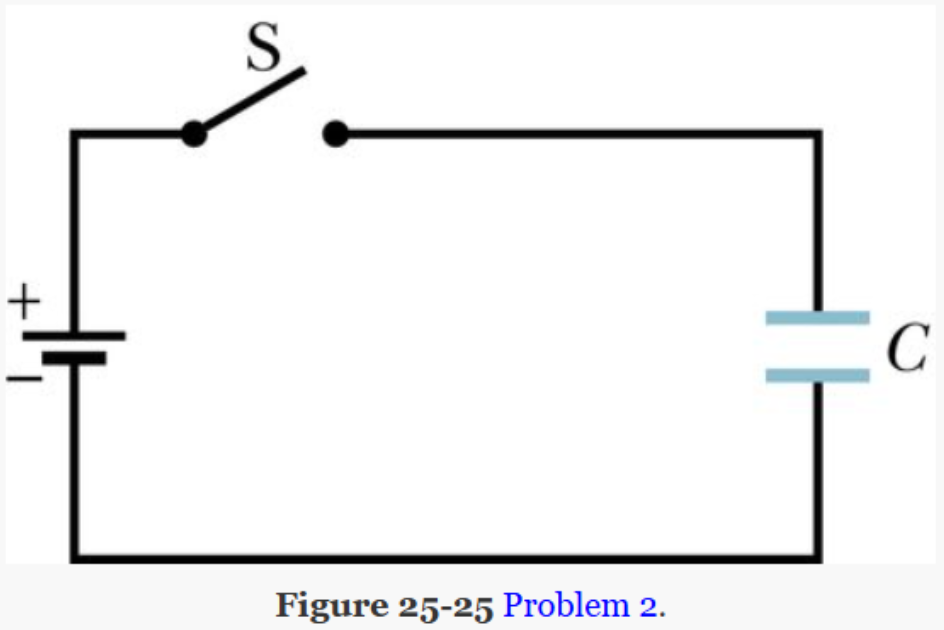
\includegraphics[width=0.25\textwidth]{picture_1.png} 
%     % \label{fig:wrapfig}
% \end{wrapfigure}

\subsection*{Solution}


\pagebreak
\section{Problem 4}
Find all six solutions to the equation $z^6 = 1$ and write each in the form $A + iB$ and plot them in the complex plane. Hint: write $z = Re^{i\theta}$ for $R$ real and positive, and find $R$ and $\theta$.
% \begin{wrapfigure}{r}{0.25\textwidth}
%     \vspace{-30pt}
%     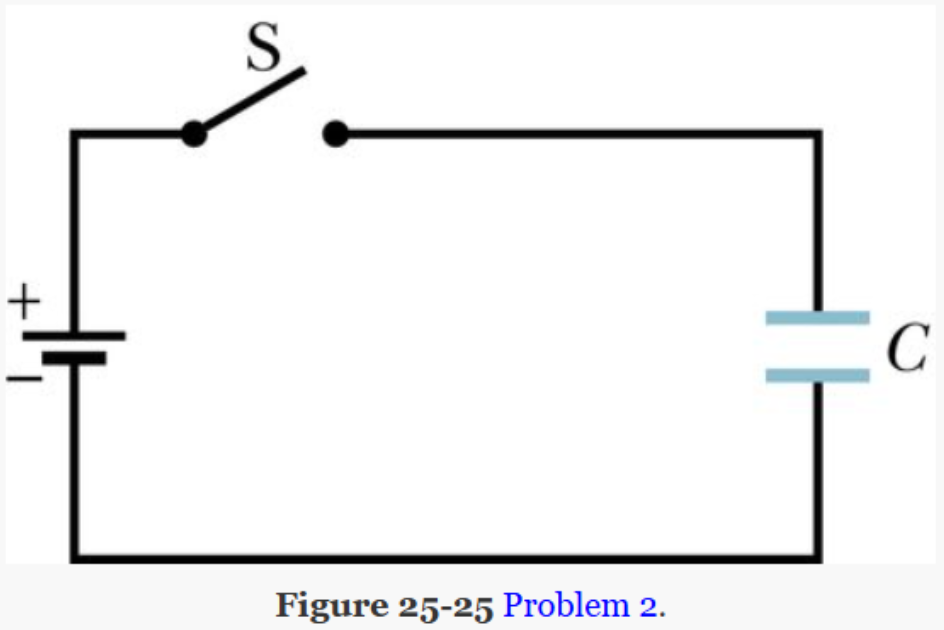
\includegraphics[width=0.25\textwidth]{picture_1.png} 
%     % \label{fig:wrapfig}
% \end{wrapfigure}


\subsection*{Solution}


\pagebreak
\section{Problem 5}
Find three independent solutions to the differential equation
\[ \frac{d^3}{dt^3} f(t) + f(t) = 0. \]
You should use complex exponentials to derive the solutions, but express the results in real
form.
% \begin{wrapfigure}{r}{0.25\textwidth}
%     \vspace{-30pt}
%     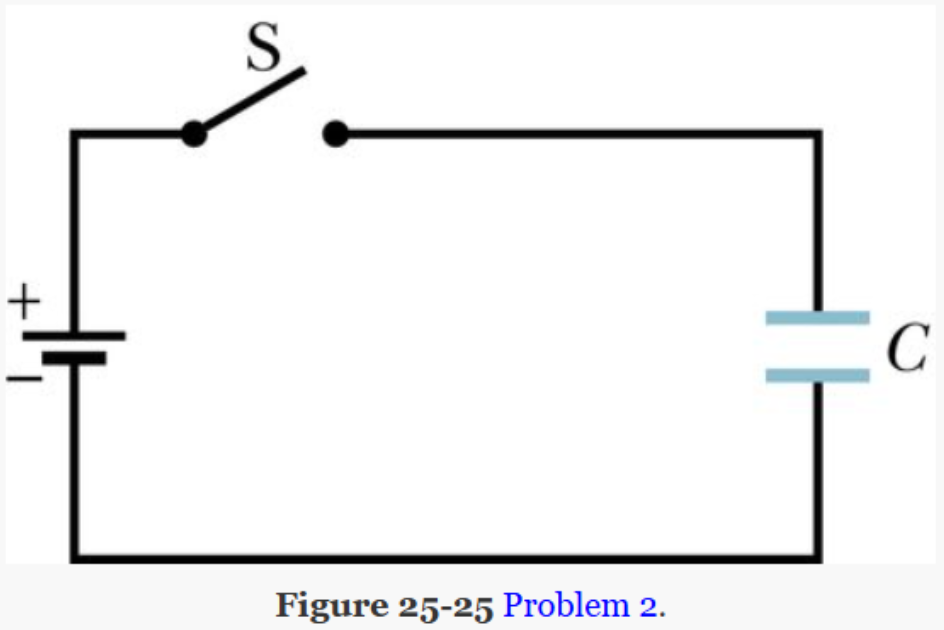
\includegraphics[width=0.25\textwidth]{picture_1.png} 
%     % \label{fig:wrapfig}
% \end{wrapfigure}


\subsection*{Solution}


\end{document}